% Drawing 79/14-3 -- folder 79, batch 14, archive page 280 (PDF page 281).
% Transcription: un losange : $u$ à gauche, $v$ à droite, $s$ en haut, $t$ en bas ; la diagonale $uv$ et les côtés marqués $A$ et $A_0$ ; suivi de trois traits verticaux.
% Kind: rhombus with its diagonal, labelled faces. Method 2 (schematic redraw from the facsimile). Status: partial.
% Notes: Rhombus u (left), s (top), v (right), t (bottom) with the diagonal uv; the four vertices are the intersections of the drawn sides (on the page each side stops short of the vertices, and s and t sit in the gaps, each with a dot); the sides and the diagonal are drawn between these points. A in each of the three triangles he marks (lower left, on the diagonal, lower right); small circles beside the upper left and upper right sides; then three vertical strokes. Still differs: the vertices t and s fall a little beyond the letters (the strokes converge loosely); the label A_0 of the transcription is not legible: at the bottom left there is a scrawl read "A d" followed by other letters, which may be text rather than a label, and A_0 is placed there after the transcription (grey). Redrawn 2026-11-09 (issue 128): to check again.
% Coordinates: 1 unit = 1 mm = 1/100 of the crop width (bbox in page fractions: [0.6, 0.5, 0.86, 0.59]).
% Redrawn by Claude (claude-opus-5-5), issue #73, 2026-11-09; not checked by a human; not compiled (no TeX in the session).
% Rights: reproduces part of the work -- behind RENDER_TRANSCRIPTS, never published by itself.
\documentclass[tikz,border=3pt]{standalone}
\usepackage{amsmath,amssymb}
\usetikzlibrary{patterns,arrows.meta}
\tikzset{pencil/.style={black!45}, struck/.style={black!35}, mark/.style={circle,draw,inner sep=1.3pt}, pt/.style={circle,fill,inner sep=0.9pt}, opt/.style={circle,draw,fill=white,inner sep=1.1pt}}
\begin{document}
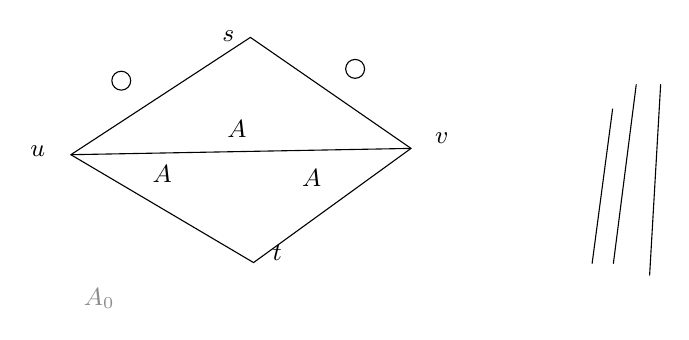
\begin{tikzpicture}[x=1mm,y=1mm,line cap=round,line join=round,font=\scriptsize]
\draw (13.4,-27.7) -- (36.2,-12.8) -- (56.6,-26.9) -- (36.6,-41.4) -- cycle;
\draw (13.4,-27.7) -- (56.6,-26.9);
\draw (19.8,-18.3) circle[radius=1.2];
\draw (49.5,-16.8) circle[radius=1.2];
\node[inner sep=1pt] at (9.2,-27.3) {\small $u$};
\node[inner sep=1pt] at (60.5,-25.6) {\small $v$};
\node[inner sep=1pt] at (33.4,-12.6) {\small $s$};
\node[inner sep=1pt] at (39.6,-40.2) {\small $t$};
\node[inner sep=1pt] at (25,-30.2) {\small $A$};
\node[inner sep=1pt] at (34.5,-24.4) {\small $A$};
\node[inner sep=1pt] at (44,-30.6) {\small $A$};
\node[inner sep=1pt,pencil] at (17,-46) {\small $A_0$};
\draw (82.2,-21.9) -- (79.6,-41.5);
\draw (85.2,-18.8) -- (82.3,-41.5);
\draw (88.3,-18.8) -- (86.9,-43);
\end{tikzpicture}
\end{document}
